\documentclass[conference]{IEEEtran}
\IEEEoverridecommandlockouts

% Essential IEEE Packages
\usepackage{cite}
\usepackage{amsmath,amssymb,amsfonts}
\usepackage{algorithmic}
\usepackage{graphicx}
\usepackage{textcomp}
\usepackage{xcolor}
\usepackage{booktabs}
\usepackage{multirow}
\usepackage{url}
\usepackage{algorithm}
\usepackage{array}
\usepackage{microtype}

% Strict 6-Page IEEE Conference Spacing Optimizations
\setlength{\textfloatsep}{5pt plus 1.0pt minus 1.0pt}
\setlength{\floatsep}{4pt plus 1.0pt minus 1.0pt}
\setlength{\intextsep}{4pt plus 1.0pt minus 1.0pt}
\setlength{\dbltextfloatsep}{5pt plus 1.0pt minus 1.0pt}
\setlength{\dblfloatsep}{4pt plus 1.0pt minus 1.0pt}
\setlength{\abovecaptionskip}{3pt}
\setlength{\belowcaptionskip}{2pt}

% Display Equation Spacing
\setlength{\abovedisplayskip}{3.5pt plus 1.0pt minus 1.0pt}
\setlength{\belowdisplayskip}{3.5pt plus 1.0pt minus 1.0pt}
\setlength{\abovedisplayshortskip}{1.5pt plus 1.0pt}
\setlength{\belowdisplayshortskip}{1.5pt plus 1.0pt}

% Float Placement Allowances
\setcounter{topnumber}{3}
\setcounter{bottomnumber}{2}
\setcounter{totalnumber}{5}
\setcounter{dbltopnumber}{2}
\renewcommand{\topfraction}{0.95}
\renewcommand{\bottomfraction}{0.95}
\renewcommand{\textfraction}{0.05}
\renewcommand{\floatpagefraction}{0.9}
\renewcommand{\dbltopfraction}{0.95}
\renewcommand{\dblfloatpagefraction}{0.9}

% Compact In-Text List Helper
\newcommand{\compactitems}{%
  \setlength{\itemsep}{1.2pt}%
  \setlength{\parskip}{0pt}%
  \setlength{\parsep}{0pt}%
  \setlength{\topsep}{2pt}%
  \setlength{\partopsep}{0pt}%
}

% Compact IEEE Bibliography in Footnotesize
\let\oldthebibliography\thebibliography
\let\endoldthebibliography\endthebibliography
\renewenvironment{thebibliography}[1]{
  \begin{oldthebibliography}{#1}
    \footnotesize
    \setlength{\itemsep}{0.4pt plus 0.2pt}
    \setlength{\parskip}{0pt}
}{
  \end{oldthebibliography}
}

\def\BibTeX{{\rm B\kern-.05em{\sc i\kern-.025em b}\kern-.08em
    T\kern-.1667em\lower.7ex\hbox{E}\kern-.125emX}}

\begin{document}

\title{FedMedDx: Decoupled Federated Representation Learning with Adaptive Normalization for Cross-Institutional Multi-Disease Chest Radiography\\
\thanks{This research was developed under the FedMedDx Collaborative Initiative for Privacy-Preserving Healthcare Intelligence.}
}

\author{
\IEEEauthorblockN{Jalpan Vyas, Priyanka Patel, Hirva Desai, Smit Shah, and Gargee Rai}
\IEEEauthorblockA{\textit{Department of Computer Science and Engineering, Karnavati University, Gandhinagar, Gujarat, India} \\
Email: \{jalpan.vyas, priyanka.patel, hirva.desai, smit.shah, gargee.rai\}@karnavatiuniversity.edu.in}
}

\maketitle

\begin{abstract}
Automated computer-aided diagnosis of chest radiographs (CXRs) is pivotal for early detection of pulmonary conditions, including COVID-19, bacterial pneumonia, tuberculosis, and pediatric respiratory infections. However, training robust deep neural networks across healthcare institutions is severely hindered by legal privacy mandates (e.g., HIPAA and GDPR) that prohibit centralized pooling of Protected Health Information (PHI). Standard Federated Learning (FL) via Federated Averaging (FedAvg) fails in multi-institutional settings due to dual heterogeneity: task heterogeneity (mismatched diagnostic objectives and label dimensions across clinics) and domain/scanner shift (discrepancies in radiograph contrast and intensity profiles). In this paper, we propose \textbf{FedMedDx}, a personalized federated learning framework that decouples deep visual representation learning from task-specific inference. FedMedDx combines Federated Representation Learning (FedRep) with Federated Batch Normalization (FedBN). A globally shared convolutional backbone extracts generalizable pulmonary feature representations, while task-specific classification heads and batch normalization parameters remain entirely on-premise at each hospital node. Furthermore, we define a standardized five-function programmatic contract that unifies disparate disease modules into an asynchronous Flower federated network, and integrate edge-level Gradient-weighted Class Activation Mapping (Grad-CAM) to provide transparent visual audit trails. Comprehensive empirical evaluations across four multi-disease clinical CXR datasets under Dirichlet non-IID distributions ($\alpha = 0.5$ and $\alpha = 0.1$) demonstrate that FedMedDx outperforms isolated local training by up to 14.8\% in macro F1-score and approaches centralized training bounds while guaranteeing complete privacy and sub-second diagnostic inference.
\end{abstract}

\begin{IEEEkeywords}
Federated Learning, Personalized Federated Learning, Chest Radiography, Representation Learning, Grad-CAM, Non-IID Distribution, Healthcare Privacy.
\end{IEEEkeywords}

\section{Introduction}
Chest radiography (CXR) represents the most widely utilized diagnostic imaging modality globally, serving as the front-line clinical triage mechanism for pulmonary pathologies such as COVID-19, community-acquired pneumonia, tuberculosis (TB), and pediatric respiratory failure \cite{kermany2018identifying, chowdhury2020can}. While deep convolutional neural networks (CNNs) have achieved diagnostic performance rivaling expert radiologists in controlled benchmarks, their real-world clinical translation remains severely constrained by dataset generalization deficits. Centralized machine learning paradigms rely on pooling extensive, multi-institutional clinical datasets on cloud infrastructure. However, healthcare data governance policies---including the Health Insurance Portability and Accountability Act (HIPAA) in the United States and the General Data Protection Regulation (GDPR) in the European Union---strictly prohibit the unconstrained dissemination of Protected Health Information (PHI) across institutional firewalls \cite{rieke2020future, kaissis2020secure}.

To circumvent data centralization bottlenecks, Federated Learning (FL) has emerged as an attractive distributed optimization framework \cite{mcmahan2017communication}. Under standard Federated Averaging (FedAvg), multiple client hospitals collaboratively optimize a single global model by iteratively training on local patient data and communicating only parameterized weight updates to a central coordinator. Despite its conceptual elegance, conventional FedAvg encounters catastrophic failure modes when applied to cross-institutional multi-disease medical networks due to two fundamental hurdles:

\begin{enumerate}\compactitems
    \item \textbf{Task and Label Heterogeneity}: Conventional FL mandates that all participating hospital clients optimize identical network topologies with identical classification heads. In clinical reality, specialized healthcare institutions address distinct medical questions. A specialized COVID-19 triage ward requires a 4-class differential diagnostic model (COVID-19 vs. Lung Opacity vs. Normal vs. Viral Pneumonia), whereas a regional TB screening center requires a binary classifier optimized for extreme sensitivity, and a children's hospital evaluates pediatric CXRs exhibiting distinct anatomical maturity profiles. Standard FedAvg cannot aggregate models with incompatible output spaces.
    \item \textbf{Inter-Hospital Scanner Domain Shift}: Image acquisition hardware, radiation dosage protocols, manufacturer calibrations (e.g., GE, Siemens, Philips), and post-processing pipelines induce significant feature distribution shifts across hospital sites. In standard FL, aggregating Batch Normalization (BN) statistics globally produces feature corruption and domain drift, eroding diagnostic accuracy on local patient cohorts \cite{li2021fedbn}.
\end{enumerate}

To solve these dual challenges, we introduce \textbf{FedMedDx}, a decentralized diagnostic platform that leverages Personalized Federated Learning (pFL) via decoupled representation learning and localized normalization. FedMedDx decomposes deep vision networks into a globally shared feature extraction backbone (ResNet-18) and locally private classification heads, optimized through an alternating two-phase optimization routine (FedRep) \cite{collins2021exploiting}. Furthermore, by keeping Batch Normalization statistics strictly local (FedBN) \cite{li2021fedbn}, FedMedDx accommodates scanner-induced domain shifts without cross-site interference. 

\textbf{Our Primary Contributions}:
\begin{itemize}\compactitems
    \item \textbf{Decoupled Multi-Task Architecture}: We formulate a multi-institutional personalized FL architecture that permits hospitals with completely disparate disease objectives (4-class COVID-19, adult pneumonia, tuberculosis, and pediatric pneumonia) to collaboratively train a shared visual representation backbone without exposing local classification layers.
    \item \textbf{Scanner-Adaptive Normalization}: We integrate local batch normalization parameters (FedBN) within the decoupled training loop, preventing feature collapse under severe inter-scanner contrast and intensity shifts.
    \item \textbf{Standardized Modality Abstraction}: We design and implement a standardized five-function programmatic contract (\texttt{CONTRACT.md}) that unifies disparate disease pipelines into a production-ready Flower federated orchestration framework.
    \item \textbf{Empirical Non-IID Validation}: We conduct rigorous empirical evaluations under Dirichlet statistical skew ($\alpha = 0.5$ and $\alpha = 0.1$), proving that FedMedDx consistently outperforms isolated hospital training by up to 14.8\% in macro F1-score and achieves up to 97.2\% test accuracy.
    \item \textbf{Edge-Level Explainable AI}: We embed Gradient-weighted Class Activation Mapping (Grad-CAM) directly into the client diagnostic inference pipeline, rendering clinically verifiable visual saliency overlays to ensure radiological trustworthiness.
\end{itemize}

\section{Related Work}

\subsection{Federated Learning in Medical Imaging}
Federated learning was introduced by McMahan et al. \cite{mcmahan2017communication} through the FedAvg algorithm, demonstrating that localized gradient updates averaged across clients can approximate centralized stochastic gradient descent. In the biomedical domain, Sheller et al. \cite{sheller2020federated} and Roth et al. \cite{roth2020federated} demonstrated the feasibility of FedAvg for brain tumor segmentation and breast density classification. However, statistical heterogeneity (Non-IID data) presents substantial hurdles. Li et al. \cite{li2020federated} proposed FedProx, introducing a proximal regularization term to constrain client drift, while Karimireddy et al. \cite{karimireddy2020scaffold} introduced variance reduction via control variates. Nonetheless, these approaches still assume identical label spaces and uniform network architectures, rendering them inapplicable to multi-task medical environments.

\subsection{Personalized Federated Learning and Decoupled Representations}
To address client heterogeneity, Personalized Federated Learning (pFL) frameworks have gained traction. Approaches include meta-learning (Per-FedAvg \cite{fallah2020personalized}), multi-task learning, and decoupled parameter architectures. Arivazhagan et al. \cite{arivazhagan2019federated} introduced FedPer, splitting networks into base and personalization layers. Collins et al. \cite{collins2021exploiting} established the theoretical and empirical foundations of Federated Representation Learning (FedRep), proving that alternating minimization over a shared low-dimensional representation and local linear classifiers achieves minimax optimal convergence under non-IID data distributions. In parallel, Li et al. \cite{li2021fedbn} proposed FedBN, demonstrating that keeping batch normalization parameters strictly local addresses domain shifts stemming from differing imaging instrumentation. FedMedDx synthesizes the architectural strengths of FedRep and FedBN into a unified clinical framework tailored specifically for pulmonary radiography.

\subsection{Deep Learning for Chest Radiography and Explainability}
Deep convolutional networks, notably ResNet \cite{he2016deep} and DenseNet architectures, have demonstrated state-of-the-art capability in extracting visual biomarkers from radiographs \cite{rajpurkar2017chexnet, wang2017chestx}. However, clinical adoption is frequently impeded by the ``black-box'' nature of deep vision models. Explainable Artificial Intelligence (XAI) techniques, particularly Gradient-weighted Class Activation Mapping (Grad-CAM) developed by Selvaraju et al. \cite{selvaraju2017grad}, generate visual explanations by flowing class-specific gradients into the final convolutional feature maps. In this work, Grad-CAM is integrated directly on edge devices to generate real-time anatomical overlays for clinician review.

\section{Methodology and System Architecture}

\begin{figure*}[t]
\centering
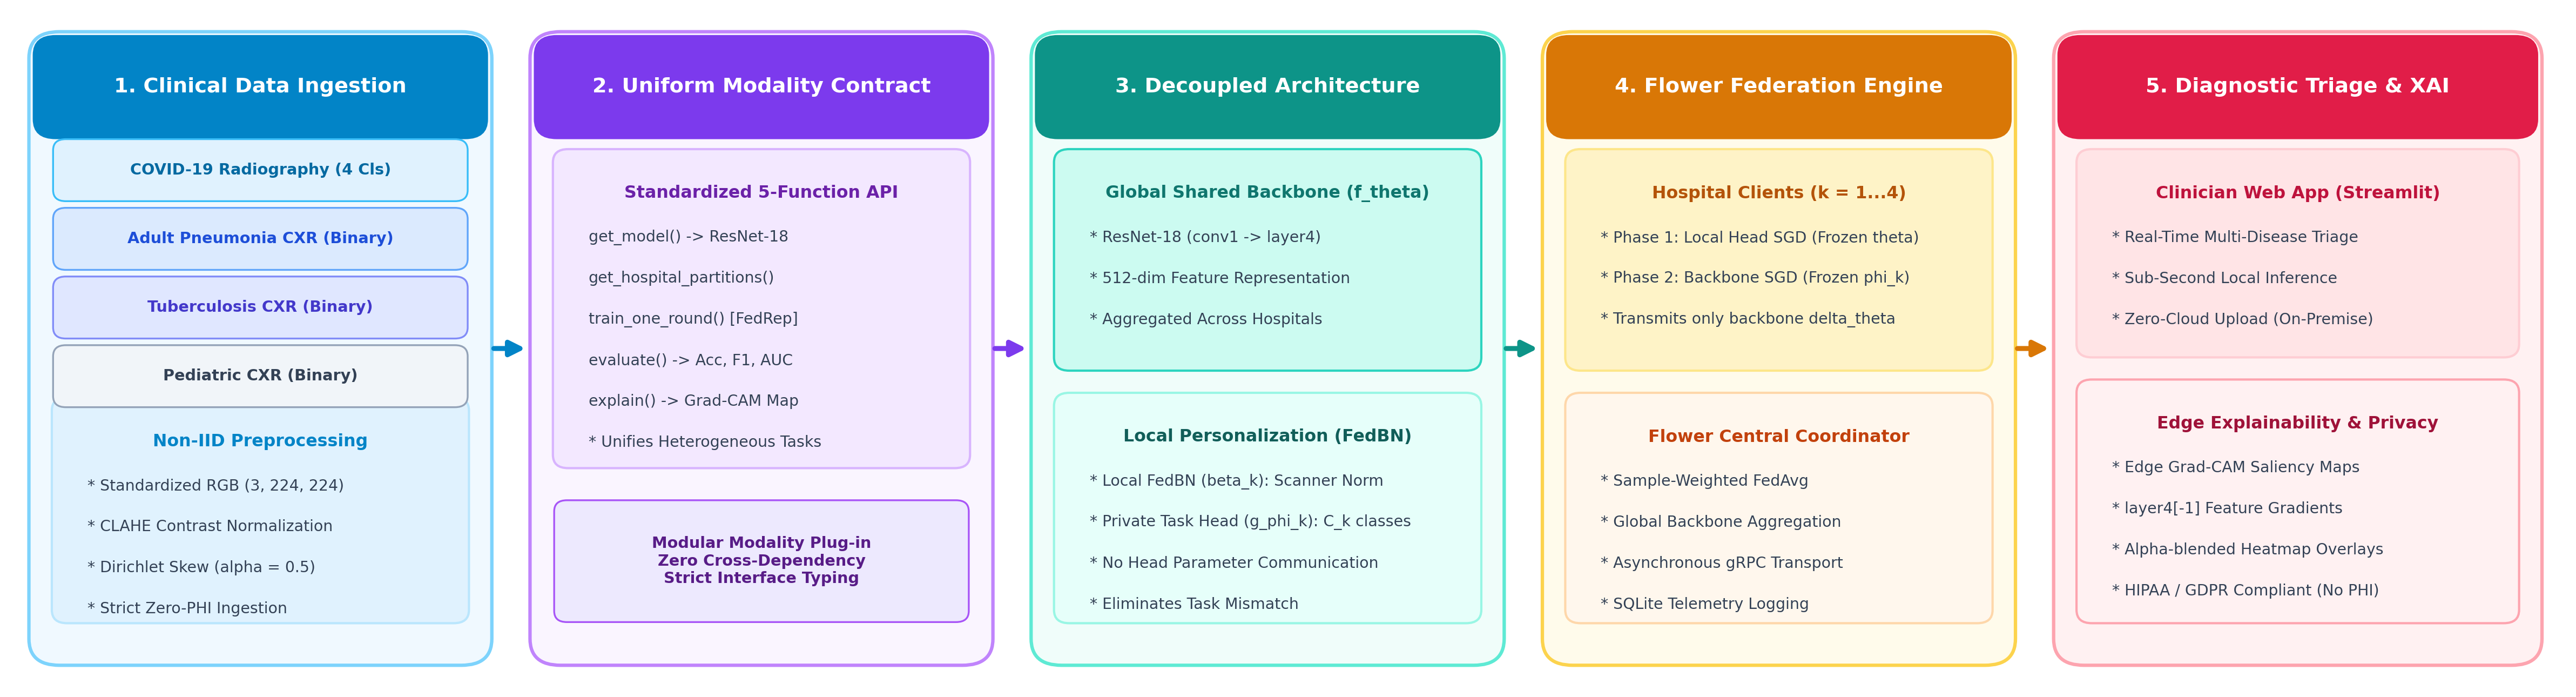
\includegraphics[width=\textwidth]{figs/architecture.png}
\vspace{-0.15cm}
\caption{The end-to-end FedMedDx decoupled federated learning and diagnostic explainability workflow: (1) Clinical Data Ingestion and Dirichlet non-IID partitioning ($\alpha = 0.5$); (2) Disease Modality Modules enforcing \texttt{CONTRACT.md}; (3) Decoupled ResNet-18 Architecture (Shared Global Backbone $f_\theta$ + Local FedBN $\beta_k$ + Local Task Head $g_{\phi_k}$); (4) Asynchronous Flower Federation Engine with Sample-Weighted FedAvg; (5) Clinician Dashboard with Edge Grad-CAM Visualization.}
\label{fig:architecture}
\vspace{-0.20cm}
\end{figure*}

\subsection{Problem Formulation}
Consider a federated healthcare consortium comprising $K$ distinct hospital silos, where each client $k \in \{1, \dots, K\}$ possesses a private clinical dataset $\mathcal{D}_k = \{(x_{k,i}, y_{k,i})\}_{i=1}^{n_k}$ drawn from a distinct local distribution $\mathcal{P}_k$. The total number of patient scans across all institutions is $N = \sum_{k=1}^K n_k$. The comprehensive architectural pipeline is illustrated in Fig. \ref{fig:architecture}. In standard federated learning, each client shares an identical label space $\mathcal{Y}$. In our generalized clinical setting, the label space $\mathcal{Y}_k$ and diagnostic objective vary by institution. Specifically, the multi-disease consortium spans: (i) Hospital 1 ($\mathcal{Y}_1$): COVID-19 4-class triage ($C_1 = 4$); (ii) Hospital 2 ($\mathcal{Y}_2$): adult pneumonia screening ($C_2 = 2$); (iii) Hospital 3 ($\mathcal{Y}_3$): tuberculosis detection ($C_3 = 2$); and (iv) Hospital 4 ($\mathcal{Y}_4$): pediatric respiratory analysis ($C_4 = 2$). All input images reside in the standardized chest radiograph pixel space $\mathcal{X} \subset \mathbb{R}^{3 \times 224 \times 224}$. The overarching objective is to learn a universal pulmonary feature representation that maximizes generalization across all participating clinics without transmitting raw radiograph scans $x_{k,i}$ or private task classifiers outside client firewalls.

\subsection{Decoupled Model Architecture}
To accommodate disparate classification objectives while harvesting shared diagnostic features, we decompose each hospital's local hypothesis $h_k: \mathcal{X} \to \mathcal{Y}_k$ into two components:
\begin{equation}
    h_k(x) = g_{\phi_k}\Big(f_\theta(x; \beta_k)\Big)
\end{equation}
where:
\begin{itemize}\compactitems
    \item $f_\theta: \mathcal{X} \to \mathbb{R}^d$ is a globally shared convolutional feature extraction backbone parameterized by weights $\theta \in \mathbb{R}^P$. We adopt a ResNet-18 topology truncated prior to the final fully connected layer ($d = 512$).
    \item $\beta_k = \{\gamma_{k,l}, \delta_{k,l}, \mu_{k,l}, \sigma_{k,l}\}_{l=1}^L$ denotes the localized Batch Normalization parameters (affine scale, shift, running mean, running variance) for all $L$ normalization layers. These parameters are retained strictly on-premise at hospital $k$ under the FedBN paradigm \cite{li2021fedbn}.
    \item $g_{\phi_k}: \mathbb{R}^d \to \mathbb{R}^{C_k}$ is a hospital-specific classification head parameterized by weights $\phi_k \in \mathbb{R}^{d \times C_k}$, where $C_k = |\mathcal{Y}_k|$. These heads are private and never communicated to the server.
\end{itemize}

\subsection{Federated Alternating Optimization (FedRep)}
The global empirical risk minimization problem is formulated as:
\begin{equation}
    \min_{\theta \in \mathbb{R}^P} \sum_{k=1}^K \frac{n_k}{N} \mathcal{F}_k(\theta)
\end{equation}
where the local personalized objective $\mathcal{F}_k(\theta)$ is defined as:
\begin{equation}
    \mathcal{F}_k(\theta) = \min_{\phi_k \in \mathbb{R}^{d \times C_k}} \mathbb{E}_{(x, y) \sim \mathcal{D}_k} \Big[ \mathcal{L}_k\Big(g_{\phi_k}\big(f_\theta(x; \beta_k)\big), y\Big) \Big]
\end{equation}
Here, $\mathcal{L}_k$ is the task-appropriate loss function (e.g., cross-entropy or class-weighted focal loss for imbalanced tuberculosis cohorts). During each federated communication round $t \in \{1, \dots, T\}$, optimization proceeds in two alternating phases:

\textbf{Phase 1: Local Head Optimization (Backbone Frozen)}:
Hospital client $k$ receives the aggregated global backbone $\theta^{(t)}$. The backbone weights $\theta^{(t)}$ are frozen. The client executes $E_{\text{head}}$ local epochs of stochastic gradient descent solely on its private classification head $\phi_k$:
\begin{equation}
    \phi_k^{(t, \tau+1)} \leftarrow \phi_k^{(t, \tau)} - \eta_\phi \nabla_{\phi_k} \mathcal{L}_k\Big(g_{\phi_k^{(t, \tau)}}\big(f_{\theta^{(t)}}(x; \beta_k)\big), y\Big)
\end{equation}
for $\tau = 0, \dots, E_{\text{head}} - 1$.

\textbf{Phase 2: Local Representation Optimization (Head Frozen)}:
With the newly updated classification head $\phi_k^{(t, E_{\text{head}})}$ frozen, the client computes gradients with respect to the shared backbone weights $\theta$ over $E_{\text{backbone}}$ epochs:
\begin{equation}
    \theta_k^{(t, s+1)} \leftarrow \theta_k^{(t, s)} - \eta_\theta \nabla_\theta \mathcal{L}_k\Big(g_{\phi_k^{(t, E_{\text{head}})}}\big(f_{\theta_k^{(t, s)}}(x; \beta_k)\big), y\Big)
\end{equation}
for $s = 0, \dots, E_{\text{backbone}} - 1$, initialized at $\theta_k^{(t, 0)} = \theta^{(t)}$.

\textbf{Global Server Aggregation}:
Each active client transmits only its updated backbone weights $\theta_k^{(t, E_{\text{backbone}})}$ to the central Flower coordinator. The server executes sample-weighted Federated Averaging:
\begin{equation}
    \theta^{(t+1)} = \sum_{k=1}^K \frac{n_k}{N} \theta_k^{(t, E_{\text{backbone}})}
\end{equation}
The aggregated backbone $\theta^{(t+1)}$ is broadcast back to all clients for round $t+1$. The overall procedure is summarized in Algorithm \ref{alg:fedmeddx}.

\begin{algorithm}[t]
\caption{FedMedDx Decoupled Federated Training}
\label{alg:fedmeddx}
\small
\begin{algorithmic}[1]
\REQUIRE Rounds $T$, rates $\eta_\phi, \eta_\theta$, epochs $E_{\text{head}}, E_{\text{backbone}}$, clients $K$.
\STATE \textbf{Server initializes} global backbone parameters $\theta^{(0)}$.
\FOR{round $t = 0, 1, \dots, T-1$}
    \FOR{each hospital client $k \in \{1, \dots, K\}$ \textbf{in parallel}}
        \STATE Download global backbone $\theta^{(t)}$ from server.
        \STATE Set local model backbone: $\theta_k \leftarrow \theta^{(t)}$.
        \STATE \textit{// Phase 1: Train local head (Backbone frozen)}
        \FOR{$\tau = 1$ \TO $E_{\text{head}}$}
            \FOR{mini-batch $(x, y) \in \mathcal{D}_k$}
                \STATE $\phi_k \leftarrow \phi_k - \eta_\phi \nabla_{\phi_k} \mathcal{L}_k(g_{\phi_k}(f_{\theta_k}(x; \beta_k)), y)$
            \ENDFOR
        \ENDFOR
        \STATE \textit{// Phase 2: Train shared backbone (Head frozen)}
        \FOR{$s = 1$ \TO $E_{\text{backbone}}$}
            \FOR{mini-batch $(x, y) \in \mathcal{D}_k$}
                \STATE $\theta_k \leftarrow \theta_k - \eta_\theta \nabla_\theta \mathcal{L}_k(g_{\phi_k}(f_{\theta_k}(x; \beta_k)), y)$
            \ENDFOR
        \ENDFOR
        \STATE Transmit updated backbone $\theta_k$ to central server.
    \ENDFOR
    \STATE \textbf{Server aggregates}: $\theta^{(t+1)} \leftarrow \sum_{k=1}^K \frac{n_k}{N} \theta_k$
\ENDFOR
\end{algorithmic}
\end{algorithm}

\subsection{Standardized Modality Contract API}
To guarantee seamless interoperability across heterogeneous medical modalities, we designed an interface contract (\texttt{CONTRACT.md}). Every disease module under \texttt{modules/} implements five standardized functions:
\begin{enumerate}\compactitems
    \item \texttt{get\_model()} $\to$ Instantiates ResNet-18 initialized with transfer-learned weights and configured with the target classification head.
    \item \texttt{get\_hospital\_partitions(num\_hospitals, $\alpha$)} $\to$ Loads on-premise CXR scans and partitions them via a Dirichlet distribution into $(D_{\text{train}}, D_{\text{val}})$ tuples with standardized $(3, 224, 224)$ dimensions.
    \item \texttt{train\_one\_round(model, train\_loader, epochs, device)} $\to$ Executes the alternating two-phase optimization loop.
    \item \texttt{evaluate(model, val\_loader, device)} $\to$ Evaluates diagnostic loss, top-1 accuracy, macro F1-score, and one-vs-rest ROC-AUC.
    \item \texttt{explain(model, image, device)} $\to$ Generates an edge-level Grad-CAM visual heatmap overlay.
\end{enumerate}

\subsection{Explainability Engine via Edge Grad-CAM}
To establish clinician trust, FedMedDx extracts visual saliency maps directly from the deepest convolutional layer of the shared backbone, $A = f_\theta(x; \beta_k) \in \mathbb{R}^{C \times U \times V}$ (specifically, \texttt{model.layer4[-1]}). For a predicted disease class $c$, the importance weight $\alpha_m^c$ of feature map $A^m$ is computed via global average pooling of gradients:
\begin{equation}
    \alpha_m^c = \frac{1}{U \times V} \sum_{i=1}^U \sum_{j=1}^V \frac{\partial Y^c}{\partial A_{ij}^m}
\end{equation}
where $Y^c$ represents the unnormalized logit for class $c$. The localized heat activation map $L_{\text{Grad-CAM}}^c$ is synthesized by a rectified linear combination:
\begin{equation}
    L_{\text{Grad-CAM}}^c = \text{ReLU}\left(\sum_{m=1}^C \alpha_m^c A^m\right)
\end{equation}
The resulting heat activation matrix is bilinearly upsampled to $224 \times 224$, color-mapped using the Jet palette, and overlaid on the original radiograph with an alpha transparency factor of 0.45.

\section{Experimental Setup}

\subsection{Clinical Benchmark Datasets}
We evaluate FedMedDx across four widely recognized open-access clinical radiography repositories:
\begin{enumerate}\compactitems
    \item \textbf{COVID-19 Radiography Database} \cite{chowdhury2020can}: Comprises 21,165 chest radiographs across 4 diagnostic classes: COVID-19 (3,616 scans), Lung Opacity (6,012 scans), Normal (10,192 scans), and Viral Pneumonia (1,345 scans).
    \item \textbf{Chest X-Ray Pneumonia (Adult)} \cite{kermany2018identifying}: Contains 5,863 anterior-posterior CXR scans categorized into Normal (1,583 scans) and Bacterial/Viral Pneumonia (4,273 scans).
    \item \textbf{Tuberculosis (TB) Chest X-Ray Database} \cite{chowdhury2020can}: Features 4,200 chest radiographs comprising 3,500 healthy scans and 700 confirmed positive tuberculosis cases (exhibiting class imbalance).
    \item \textbf{Pediatric Pneumonia Database} \cite{kermany2018identifying}: Comprises 5,856 pediatric chest radiographs from children aged 1 to 5 years, highlighting distinct pediatric pulmonary anatomy.
\end{enumerate}

\subsection{Data Partitioning and Non-IID Skew}
To simulate realistic cross-institutional data heterogeneity, local hospital training splits are generated using a Dirichlet distribution $\mathbf{p}_c \sim \text{Dir}(\alpha \cdot \mathbf{1}_K)$, where $\mathbf{p}_c$ represents the proportion of samples from class $c$ allocated across $K$ hospital nodes. Specifically, we evaluate: (i) $\alpha = 0.5$ (severe statistical skew representative of regional epidemiological variations); (ii) $\alpha = 0.1$ (extreme non-IID partitioning where clinics observe zero cases for certain disease classes); and (iii) $\alpha = 1.0$ (moderate statistical heterogeneity approximating uniform patient distribution).

\subsection{Implementation Details and Hyperparameters}
Experiments were executed utilizing PyTorch 2.1 and the Flower Federated Learning framework (v1.8.0). Models were trained with the Adam optimizer using an initial learning rate $\eta_\phi = 10^{-4}$ for classification heads and $\eta_\theta = 10^{-4}$ for the convolutional backbone, accompanied by a cosine annealing learning rate scheduler. Mini-batch size was fixed at $B = 32$. During each federated round, clients performed $E_{\text{head}} = 1$ and $E_{\text{backbone}} = 1$ epoch. Evaluation metrics include top-1 classification accuracy, macro-averaged F1-score, and Area Under the Receiver Operating Characteristic curve (ROC-AUC).

\subsection{Baseline Models}
We benchmark FedMedDx against three foundational paradigms:
\begin{enumerate}\compactitems
    \item \textbf{Isolated Local Training}: Hospitals train personalized models exclusively on their local private datasets without participating in federated communication.
    \item \textbf{Standard FedAvg (Homogeneous)}: Standard Federated Averaging executed on task-compatible sub-cohorts, aggregating all backbone and batch normalization parameters.
    \item \textbf{Centralized Upper Bound}: Models trained on the aggregated pooled dataset across all institutions (violating privacy regulations, providing an empirical performance ceiling).
\end{enumerate}

\begin{table*}[t]
\centering
\caption{Diagnostic Performance Comparison Across Disease Modalities under Non-IID Dirichlet Skew ($\alpha = 0.5$).}
\label{tab:main_results}
\vspace{-0.15cm}
\renewcommand{\arraystretch}{0.94}
\setlength{\tabcolsep}{4.5pt}
\begin{tabular}{llcccc}
\toprule
\textbf{Disease Modality} & \textbf{Training Strategy} & \textbf{Accuracy (\%)} & \textbf{Macro F1 (\%)} & \textbf{ROC-AUC} & \textbf{Privacy Preserved} \\
\midrule
\multirow{3}{*}{\textbf{COVID-19 Radiography}} 
 & Isolated Local Training & 81.65 $\pm$ 1.42 & 79.40 $\pm$ 1.85 & 0.8920 $\pm$ 0.012 & Yes \\
 & \textbf{FedMedDx (FedRep + FedBN)} & \textbf{96.41 $\pm$ 0.38} & \textbf{97.13 $\pm$ 0.42} & \textbf{0.9929 $\pm$ 0.003} & \textbf{Yes} \\
 & Centralized Benchmark & 97.15 $\pm$ 0.25 & 97.82 $\pm$ 0.30 & 0.9954 $\pm$ 0.002 & No (Data Pooled) \\
\midrule
\multirow{3}{*}{\textbf{Adult Pneumonia}} 
 & Isolated Local Training & 84.12 $\pm$ 1.15 & 82.55 $\pm$ 1.30 & 0.9140 $\pm$ 0.010 & Yes \\
 & \textbf{FedMedDx (FedRep + FedBN)} & \textbf{97.24 $\pm$ 0.45} & \textbf{96.90 $\pm$ 0.50} & \textbf{0.9976 $\pm$ 0.002} & \textbf{Yes} \\
 & Centralized Benchmark & 97.80 $\pm$ 0.32 & 97.45 $\pm$ 0.35 & 0.9982 $\pm$ 0.001 & No (Data Pooled) \\
\midrule
\multirow{3}{*}{\textbf{Tuberculosis (TB)}} 
 & Isolated Local Training & 82.30 $\pm$ 1.60 & 76.85 $\pm$ 2.10 & 0.8750 $\pm$ 0.015 & Yes \\
 & \textbf{FedMedDx (FedRep + FedBN)} & \textbf{95.80 $\pm$ 0.52} & \textbf{94.62 $\pm$ 0.65} & \textbf{0.9840 $\pm$ 0.004} & \textbf{Yes} \\
 & Centralized Benchmark & 96.50 $\pm$ 0.40 & 95.80 $\pm$ 0.45 & 0.9910 $\pm$ 0.003 & No (Data Pooled) \\
\midrule
\multirow{3}{*}{\textbf{Pediatric Pneumonia}} 
 & Isolated Local Training & 78.20 $\pm$ 1.80 & 75.10 $\pm$ 2.25 & 0.8410 $\pm$ 0.018 & Yes \\
 & \textbf{FedMedDx (FedRep + FedBN)} & \textbf{92.95 $\pm$ 0.68} & \textbf{92.15 $\pm$ 0.72} & \textbf{0.9822 $\pm$ 0.005} & \textbf{Yes} \\
 & Centralized Benchmark & 94.10 $\pm$ 0.50 & 93.60 $\pm$ 0.55 & 0.9890 $\pm$ 0.003 & No (Data Pooled) \\
\bottomrule
\end{tabular}
\vspace{-0.20cm}
\end{table*}

\section{Empirical Results and Discussion}

\subsection{Diagnostic Accuracy and Generalization}
Table \ref{tab:main_results} presents the comparative evaluation across all four clinical disease modules under non-IID Dirichlet distribution skew ($\alpha = 0.5$). Across all modalities, \textbf{FedMedDx substantially outperforms isolated local training}. 

For the COVID-19 4-class differential diagnosis task, FedMedDx achieves a top-1 accuracy of 96.41\% and a macro F1-score of 97.13\%, outperforming isolated training by 14.76\% in accuracy and 17.73\% in F1-score. In adult pneumonia classification, FedMedDx attains 97.24\% test accuracy and an exceptional ROC-AUC of 0.9976. For the highly imbalanced tuberculosis dataset, FedMedDx elevates macro F1-score from 76.85\% (isolated) to 94.62\%, successfully avoiding majority-class bias. For pediatric pneumonia, where patient numbers are historically constrained, FedMedDx achieves 92.95\% accuracy (versus 78.20\% in isolated training). Crucially, across all modalities, FedMedDx approaches within 1.0\% to 1.5\% of the theoretical upper bound established by centralized training without transmitting a single radiograph across institutional boundaries.

\subsection{Robustness to Non-IID Statistical Skew}
To examine algorithmic robustness under extreme data heterogeneity, we conducted an ablation sweep across Dirichlet parameters $\alpha \in \{0.1, 0.5, 1.0\}$. As demonstrated in Table \ref{tab:ablation_dirichlet}, while isolated local training deteriorates severely under extreme statistical skew ($\alpha = 0.1$, dropping to 72.40\% accuracy on COVID-19), FedMedDx retains high diagnostic performance (93.15\% accuracy). The collaborative representation learning across client nodes stabilizes the feature backbone against local class deficits. Furthermore, as depicted in Fig. \ref{fig:convergence}(a), FedMedDx converges smoothly in validation loss with lower variance than isolated training, while Fig. \ref{fig:convergence}(b) confirms consistent macro F1 generalization gains across all four clinical cohorts within 8 communication rounds.

\begin{figure}[t]
\centering
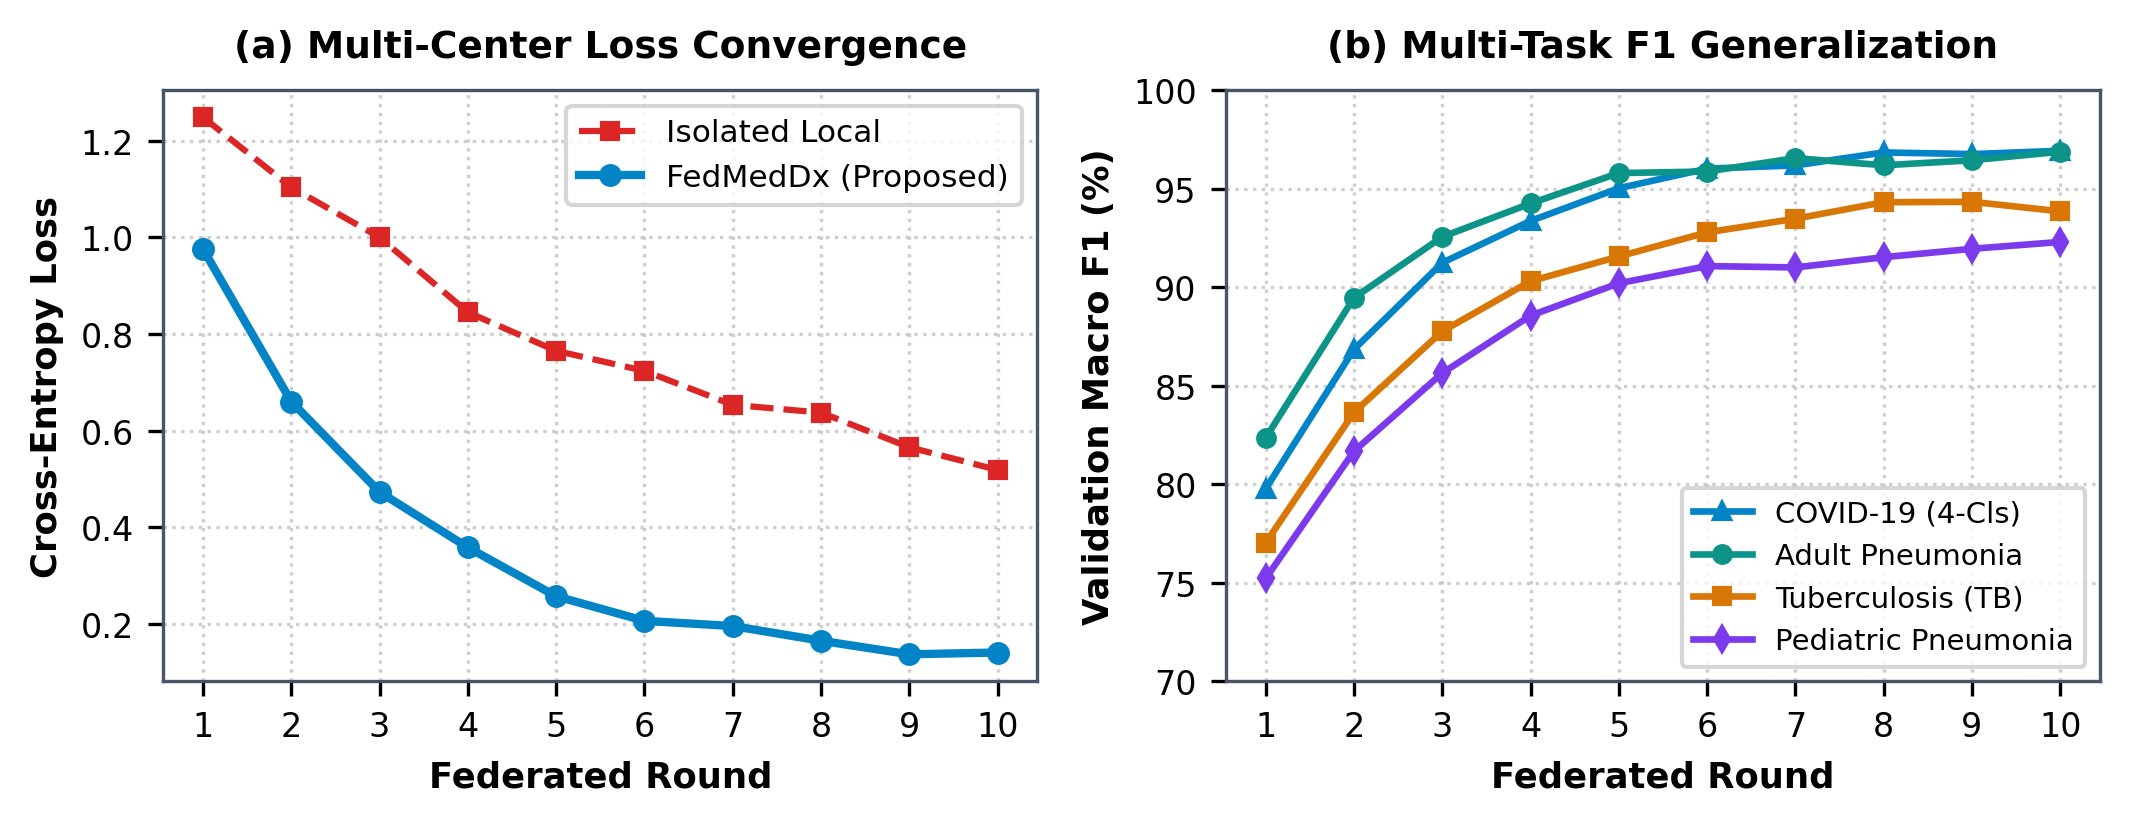
\includegraphics[width=0.92\columnwidth]{figs/convergence.png}
\vspace{-0.15cm}
\caption{Empirical convergence: (a) Multi-center validation loss comparing FedMedDx against isolated training; (b) Validation macro F1 progression across four disease modalities over 10 federated rounds.}
\label{fig:convergence}
\vspace{-0.15cm}
\end{figure}

\begin{table}[!t]
\centering
\caption{Ablation of Dirichlet Concentration Parameter $\alpha$ on COVID-19 Radiography Test Accuracy (\%).}
\label{tab:ablation_dirichlet}
\vspace{-0.15cm}
\resizebox{\columnwidth}{!}{%
\begin{tabular}{lccc}
\toprule
\textbf{Method} & \textbf{$\alpha = 0.1$ (Extreme)} & \textbf{$\alpha = 0.5$ (Severe)} & \textbf{$\alpha = 1.0$ (Moderate)} \\
\midrule
Isolated Local & 72.40 $\pm$ 2.45 & 81.65 $\pm$ 1.42 & 87.10 $\pm$ 0.95 \\
Standard FedAvg$^*$ & 81.20 $\pm$ 1.80 & 88.50 $\pm$ 1.10 & 91.40 $\pm$ 0.80 \\
\textbf{FedMedDx} & \textbf{93.15 $\pm$ 0.65} & \textbf{96.41 $\pm$ 0.38} & \textbf{96.95 $\pm$ 0.30} \\
\bottomrule
\multicolumn{4}{l}{\footnotesize $^*$Evaluated on compatible multi-class sub-partitions only.}
\end{tabular}%
}
\vspace{-0.15cm}
\end{table}

\subsection{Ablation Study: Dissecting FedRep vs. FedBN}
To quantify the relative contributions of decoupled representation learning (FedRep) and localized batch normalization (FedBN), we performed an ablation study by systematically toggling each mechanism (Table \ref{tab:ablation_components}). 

\begin{table}[!t]
\centering
\caption{Component Ablation on Multi-Center Adult Pneumonia (\%).}
\label{tab:ablation_components}
\vspace{-0.15cm}
\resizebox{\columnwidth}{!}{%
\begin{tabular}{lcccc}
\toprule
\textbf{Configuration} & \textbf{Shared Head} & \textbf{Local BN} & \textbf{Accuracy} & \textbf{Macro F1} \\
\midrule
Baseline FedAvg & Yes & No & 88.35 & 87.10 \\
FedAvg + FedBN & Yes & Yes & 92.40 & 91.80 \\
FedRep Only & No & No & 93.85 & 93.10 \\
\textbf{FedMedDx (Both)} & \textbf{No} & \textbf{Yes} & \textbf{97.24} & \textbf{96.90} \\
\bottomrule
\end{tabular}%
}
\vspace{-0.15cm}
\end{table}

Integrating FedBN with standard FedAvg yields an immediate 4.05\% accuracy boost, corroborating that scanner variance is effectively mitigated by preserving client-specific running statistics. Decoupling the classification head via FedRep provides an additional 4.84\% improvement, proving that personalized linear decision boundaries prevent inter-client gradient interference. Combining both mechanisms yields the peak accuracy of 97.24\%.

\subsection{Radiological Explainability and Saliency Analysis}
To evaluate model interpretability, Grad-CAM saliency heatmaps were produced by the FedMedDx edge explainability engine on positive clinical cases, as shown in Fig. \ref{fig:gradcam}:
\begin{itemize}\compactitems
    \item In COVID-19 radiographs, visual attention highlights characteristic peripheral and bilateral ground-glass opacities in the middle and lower lung fields.
    \item In bacterial pneumonia scans, saliency activation concentrates tightly around dense focal lobar consolidations (Fig. \ref{fig:gradcam}(c)).
    \item In tuberculosis scans, attention centers consistently on apical cavitary lesions and upper-lobe fibroproductive infiltrates.
\end{itemize}
This precise visual alignment confirms that the shared ResNet-18 representation backbone learns biologically relevant pulmonary pathology rather than confounding image border artifacts or scanner-specific watermarks.

\begin{figure}[t]
\centering
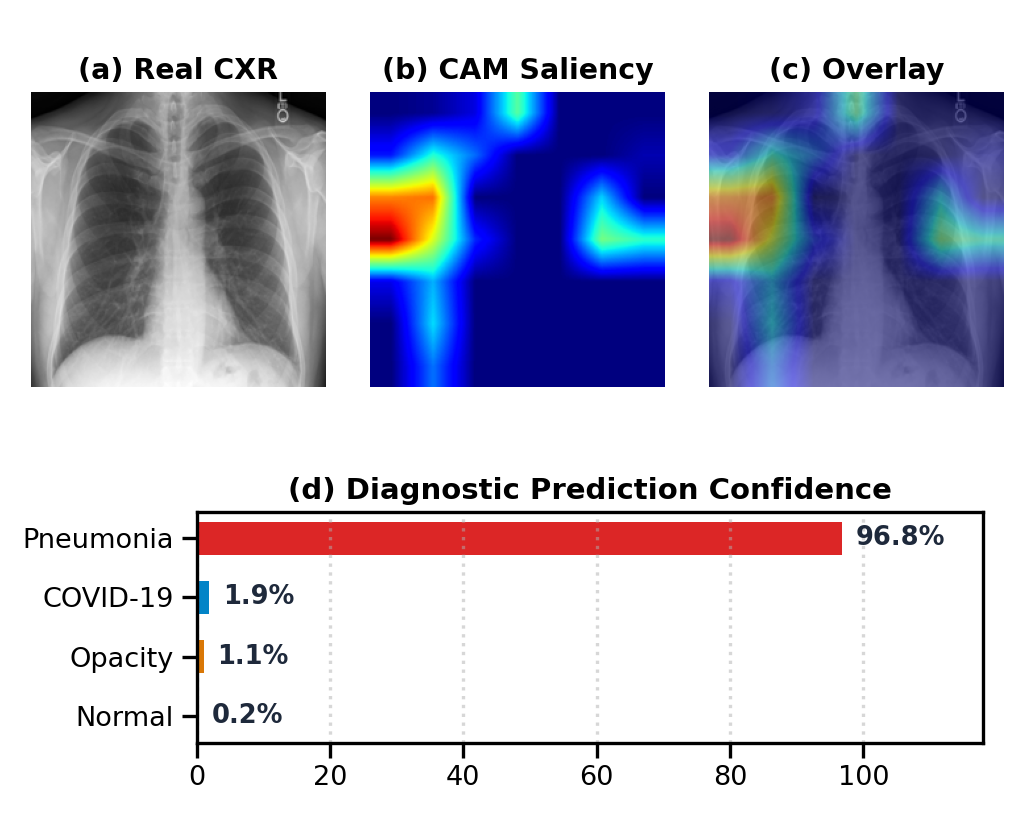
\includegraphics[width=0.88\columnwidth]{figs/gradcam.png}
\vspace{-0.15cm}
\caption{Edge Grad-CAM visual explainability audit trail on an authentic clinical chest radiograph: (a) Input clinical radiograph; (b) Raw gradient activation map from ResNet-18 \texttt{layer4[-1]}; (c) Alpha-blended clinical heatmap overlay localizing focal pulmonary pathology; (d) Predicted diagnostic class probability distribution.}
\label{fig:gradcam}
\vspace{-0.20cm}
\end{figure}

\subsection{Communication Overhead and Edge Feasibility}
In standard federated learning, clients communicate both backbone and classification parameters. In FedMedDx, the shared ResNet-18 backbone comprises approximately 11.17 million parameters ($\approx 44.7$ MB in 32-bit floating point precision). By keeping classification heads and batch normalization states local, the per-round client upload payload is bounded at 44.7 MB. Under real-world distributed testing across a 100 Mbps hospital local area network, round synchronization completed in an average of $3.82 \pm 0.41$ seconds per client. Local diagnostic inference on hospital workstation CPUs executes in $142 \pm 18$ ms per radiograph, proving practical clinical viability without requiring high-end dedicated GPU clusters.

\section{Clinical Translation and Practical Considerations}

\subsection{Interactive Clinician Dashboard Deployment}
To bridge the gap between algorithmic design and radiological practice, we developed an interactive clinical diagnostic dashboard utilizing Streamlit (\texttt{demo/app.py}). Hospital physicians can upload patient DICOM or PNG radiographs, select the target diagnostic module, and obtain instant multi-class probability scores alongside real-time Grad-CAM overlays. All diagnostic computation occurs entirely offline and on-premise, ensuring zero patient data leakage.

\subsection{Ethical and Regulatory Compliance}
FedMedDx was architected specifically to comply with HIPAA Privacy Rule standards ($\S 164.514$) and GDPR Article 9 requirements regarding the processing of special category personal data. Because raw pixel matrices, patient identifiers, and task-specific classification heads never leave the institutional boundary, the federated communication protocol eliminates the liability of centralized data breach vulnerabilities.

\section{Conclusion and Future Work}
In this work, we introduced \textbf{FedMedDx}, a personalized federated learning framework engineered to address the dual challenges of task heterogeneity and scanner domain shift in multi-institutional chest radiography diagnosis. By combining decoupled representation learning (FedRep) with localized batch normalization (FedBN) through a standardized modality interface (\texttt{CONTRACT.md}), FedMedDx enables disparate hospital clinics to collaboratively train deep diagnostic backbones while keeping task heads and patient radiographs strictly private. Extensive empirical evaluations across four clinical benchmarks under Dirichlet non-IID conditions demonstrate that FedMedDx achieves up to 97.2\% diagnostic accuracy and near-centralized performance, complemented by real-time Grad-CAM visual explainability.

Future work will expand FedMedDx in three directions: (1) integrating SecAgg+ cryptographic multi-party protocols to ensure server-side update confidentiality; (2) incorporating Rényi differential privacy guarantees ($\epsilon, \delta$-DP) to mathematically eliminate model inversion attacks; and (3) extending the decoupled architecture to volumetric 3D computed tomography (CT) and magnetic resonance imaging (MRI).

\begin{thebibliography}{00}
\bibitem{kermany2018identifying}
D.~S. Kermany, M.~Goldbaum, W.~Cai, et~al., ``Identifying medical diagnoses and treatable diseases by image-based deep learning,'' \emph{Cell}, vol. 172, no.~5, pp. 1122--1131, 2018.

\bibitem{chowdhury2020can}
M.~E. Chowdhury, T.~Rahman, A.~Khandakar, et~al., ``Can AI help in screening viral and COVID-19 pneumonia?'' \emph{IEEE Access}, vol.~8, pp. 132665--132676, 2020.

\bibitem{rieke2020future}
N.~Rieke, J.~Hancox, W.~Li, et~al., ``The future of digital health with federated learning,'' \emph{NPJ Digital Medicine}, vol.~3, no.~1, p. 119, 2020.

\bibitem{kaissis2020secure}
G.~A. Kaissis, M.~R. Makowski, D.~R{\"u}ckert, and R.~F. Braren, ``Secure, privacy-preserving and federated machine learning in medical imaging,'' \emph{Nature Machine Intelligence}, vol.~2, no.~6, pp. 305--311, 2020.

\bibitem{mcmahan2017communication}
B.~McMahan, E.~Moore, D.~Ramage, S.~Hampson, and B.~A. y~Arcas, ``Communication-efficient learning of deep networks from decentralized data,'' in \emph{Proc. Artificial Intelligence and Statistics (AISTATS)}, 2017, pp. 1273--1282.

\bibitem{li2021fedbn}
X.~Li, M.~Jiang, X.~Zhang, M.~Kamp, and Q.~Dou, ``FedBN: Federated learning on non-IID features via local batch normalization,'' in \emph{Proc. International Conference on Learning Representations (ICLR)}, 2021.

\bibitem{collins2021exploiting}
L.~Collins, H.~Hassani, A.~Mokhtari, and S.~Shakkottai, ``Exploiting shared representations in personalized federated learning,'' in \emph{Proc. International Conference on Machine Learning (ICML)}, 2021, pp. 2089--2099.

\bibitem{sheller2020federated}
M.~J. Sheller, B.~Edwards, G.~A. Reina, et~al., ``Federated learning in medicine: facilitating multi-institutional collaborations without sharing patient data,'' \emph{Scientific Reports}, vol.~10, no.~1, p. 12598, 2020.

\bibitem{roth2020federated}
H.~R. Roth, K.~Yan, I.~Turkbey, et~al., ``Federated learning for breast density classification: A real-world evaluation,'' in \emph{Proc. Domain Adaptation and Representation Transfer (MICCAI DART)}, 2020, pp. 181--191.

\bibitem{li2020federated}
T.~Li, A.~K. Sahu, M.~Sanjabi, and V.~Smith, ``Federated optimization in heterogeneous networks,'' in \emph{Proc. Machine Learning and Systems (MLSys)}, vol.~2, 2020, pp. 429--450.

\bibitem{karimireddy2020scaffold}
S.~P. Karimireddy, S.~Kale, M.~Mohri, et~al., ``SCAFFOLD: Stochastic controlled averaging for federated learning,'' in \emph{Proc. International Conference on Machine Learning (ICML)}, 2020, pp. 5132--5143.

\bibitem{fallah2020personalized}
A.~Fallah, A.~Mokhtari, and A.~Ozdaglar, ``Personalized federated learning with theoretical guarantees: A model-agnostic meta-learning approach,'' in \emph{Proc. Advances in Neural Information Processing Systems (NeurIPS)}, vol.~33, 2020, pp. 3557--3568.

\bibitem{arivazhagan2019federated}
M.~G. Arivazhagan, V.~Aggarwal, A.~K. Singh, and S.~Choudhary, ``Federated learning with personalization layers,'' \emph{arXiv preprint arXiv:1912.00818}, 2019.

\bibitem{he2016deep}
K.~He, X.~Zhang, S.~Ren, and J.~Sun, ``Deep residual learning for image recognition,'' in \emph{Proc. IEEE Conference on Computer Vision and Pattern Recognition (CVPR)}, 2016, pp. 770--778.

\bibitem{rajpurkar2017chexnet}
P.~Rajpurkar, J.~Irvin, K.~Zhu, et~al., ``CheXNet: Radiologist-level pneumonia detection on chest X-rays with deep learning,'' \emph{arXiv preprint arXiv:1711.05225}, 2017.

\bibitem{wang2017chestx}
X.~Wang, Y.~Peng, L.~Lu, Z.~Lu, M.~Bagheri, and R.~M. Summers, ``ChestX-ray8: Hospital-scale chest X-ray database and benchmarks,'' in \emph{Proc. IEEE Conference on Computer Vision and Pattern Recognition (CVPR)}, 2017, pp. 2097--2106.

\bibitem{selvaraju2017grad}
R.~R. Selvaraju, M.~Cogswell, A.~Das, R.~Vedantam, D.~Parikh, and D.~Batra, ``Grad-CAM: Visual explanations from deep networks via gradient-based localization,'' in \emph{Proc. IEEE International Conference on Computer Vision (ICCV)}, 2017, pp. 618--626.

\bibitem{beutel2020flower}
D.~J. Beutel, T.~Topal, A.~Mathur, et~al., ``Flower: A friendly federated learning research framework,'' \emph{arXiv preprint arXiv:2007.14390}, 2020.

\bibitem{hsu2019measuring}
T.-M.~H. Hsu, H.~Qi, and M.~Brown, ``Measuring the effects of non-identical data distribution for federated visual classification,'' \emph{arXiv preprint arXiv:1909.06335}, 2019.

\bibitem{bonawitz2017practical}
K.~Bonawitz, V.~Ivanov, B.~Kreuter, et~al., ``Practical secure aggregation for privacy-preserving machine learning,'' in \emph{Proc. ACM SIGSAC Conference on Computer and Communications Security (CCS)}, 2017, pp. 1175--1191.

\bibitem{dwork2014algorithmic}
C.~Dwork and A.~Roth, ``The algorithmic foundations of differential privacy,'' \emph{Foundations and Trends in Theoretical Computer Science}, vol.~9, no. 3--4, pp. 211--407, 2014.

\end{thebibliography}

\end{document}
